\documentclass[a4paper,12pt]{article}
\usepackage{amsmath, amssymb}

\usepackage[utf8]{inputenc}
%\usepackage[spanish]{babel}
\usepackage{amsmath}
\usepackage{amsfonts}
\usepackage{amssymb}
\usepackage{graphicx}
\usepackage{exercise}

\author{Pilar Barbero Iriarte}

\newenvironment{exercise}[1]% environment name
{% begin code
  \par\vspace{\baselineskip}\noindent
  \textbf{Ejercicio (#1)}\begin{itshape}%
  \par\vspace{\baselineskip}\noindent\ignorespaces
}%
{% end code
  \end{itshape}\ignorespacesafterend
}


\begin{document}

\begin{titlepage}
\begin{center}


% Upper part of the page. The '~' is needed because \\
% only works if a paragraph has started.

\textsc{\LARGE M\'aster en Modelizaci\'on \\e Investigaci\'on Matem\'atica,\\ Estad\'istica y Computaci\'on }\\[1.5cm]
{\large \today}

\textsc{Ejercicios Segunda Parte}\\[0.5cm]

% Title
\vfill

{ \huge \bfseries Modelos de Log\'istica \\[0.4cm] }

\vfill



% Author and supervisor
\noindent
\begin{minipage}{0.4\textwidth}
\begin{flushleft} \large

\includegraphics[width=1.1\textwidth]{../logoUZ.png}~\\[1cm]
\emph{Autor:}\\
Pilar Barbero Iriarte 
\end{flushleft}
\end{minipage}%
\begin{minipage}{0.4\textwidth}
\begin{flushright} \large

\includegraphics[width=0.8\textwidth]{../logoUPV.png}~\\[1cm]
\emph{Profesor:} \\
Mikel Lezaun Iturralde 
\end{flushright}
\end{minipage}

% Bottom of the page
\end{center}


\end{titlepage}

\pagebreak
\tableofcontents
\pagebreak


\section{Asignaci\'on de semanas de reserva}
\begin{exercise}{Asignaci\'on de semanas de reserva}
Contamos con un n\'umero de trabajadores: 16.

Las vacaciones est\'an dadas en el archivo: \textit{Vacaciones.xls}.\\

Durante todo el año hay 11 trabajadores con trabajo asignado. Por tanto deber\'an estar cinco de vacaciones o reserva. Como en alguna semana no hay ning\'un trabajador de vacaciones y en otras hay 2, 3 o 4 de vacaciones, para que siempre haya 11 disponibles habr\'a que asignarles semanas de reserva. Escribir un modelo de asignaci\'on de reservas lo m\'as igualatorio posible de forma que:\\

\begin{itemize}
\item[1.] Ning\'un conductor tiene m\'as de tres semanas de reserva seguidas. \\% done

\item[2.] Un conductor no puede tener una semana de reserva aislada. \\%done

\item[3.] En lo posible las semanas de reserva est\'en alejadas de las vacaciones.\\ %f objetivo
\end{itemize}

Escribir TODAS las ecuaciones necesarias para esta asignaci\'on igualitaria, no s\'olo correspondientes a las tres condiciones anteriores.\\

\end{exercise}


Sea $n\in N = \{ 1,\dots,16 \}$ el n\'umero de trabajadores y $l \in L = \{1,\dots,52\}$ el n\'umero de semanas. Vamos a definir las \textbf{variables} de forma binaria,

	\begin{equation*}
	v_{n,l} = \left\lbrace \begin{array}{l}
		1 \text{ si el conductor } n\text{-\'esimo en la semana } l \text{  tiene vacaciones,} \\
		0 \text{ si el conductor } n\text{-\'esimo en la semana } l \text{ NO tiene vacaciones.} \\
	\end{array}
	\right. 
	\end{equation*}
	

	\begin{equation*}
	y_{n,l} = \left\lbrace \begin{array}{l}
		1 \text{ si el conductor } n\text{-\'esimo en la semana } l \text{  tiene reserva,} \\
		0 \text{ si el conductor } n\text{-\'esimo en la semana } l \text{ NO tiene reserva.} \\
	\end{array}
	\right. 
	\end{equation*}
	
	
Las \textbf{restricciones} ser\'an las siguientes:\\

Aunque no se exija expl\'icitamente, si un conductor est\'a de vacaciones, no estar\'a de reserva,

$$\text{Si } v_{n,l} = 1 \text{ entonces } y_{n,l} = 0 \text{ para } n\in N, l\in L$$

Podemos observar en el fichero \textit{Vacaciones.xls} que cada trabajador tiene $9$ semanas de vacaciones,

$$ \sum_{l=1}^{52} {v_{n,l}} = 9 \text{ para } n\in N$$

Con respecto a las semanas de reserva que deber\'a realizar cada trabajador, jugando un poco con el fichero \textit{Vacaciones.xls},\\

\begin{figure}[h!]
  \centering
	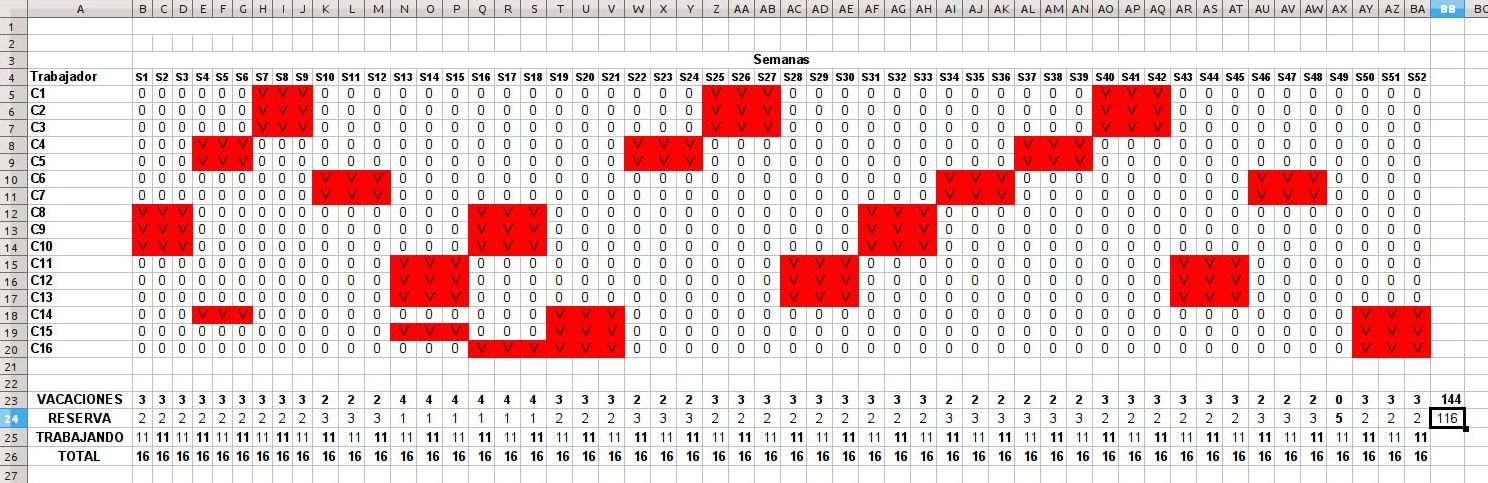
\includegraphics[scale=0.4]{reserva.png}
	  \caption{Vacaciones.xsl}
\end{figure}

Podemos observar que es necesario dividir $116$ para $16$ trabajadores disponibles, de manera que las semanas de reserva sean equitativas, as\'i que cada trabajador deber\'a realizar entre $7$ y $8$ semanas de reserva al a\~no:\\

$$ 7 \leq \sum_{l=1}^{52} {y_{n,l}} \leq 8 \text{ para } n\in N$$

Cada semana del año se encuentran $11$ trabajadores trabajando, por lo que se encontraran los restantes $6$ de vacaciones o de reserva:

$$ \sum_{n=1}^{17} (v_{n,l} + y_{n,l}) = 6 \text{ para } l = 1,\dots 52$$

\textbf{Restricci\'on 1:} Un trabajador no puede tener m\'as de tres semanas de reserva seguidas,

$$ y_{n,l} + y_{n,l+1} + y_{n,l+2} + y_{n,l+3} \leq 3 \text{ para } n\in N, \,\,l=1\dots 49$$

\textbf{Restricci\'on 2:} Un trabajador no puede tener una semana de reserva aislada,

$$ y_{n,l+1} \leq v_{n,l} + y_{n,l} + v_{n,l+2} + y_{n,l+2} \text{ para } n\in N,\,\,l = 1\dots 50$$
$$ y_{n,l} \leq y_{n,2} \text{ y } y_{n,52} \leq y_{n,51} \text{ para } n\in N$$.

\textbf{Objetivo:} El objetivo ser\'a alejar las semanas de reserva de las vacaciones:

$$ \text{min } z = \sum_{n=1}^{17}{ \sum_{\substack{l=1,\dots 49\\ v_{n,l+3}=1\\ v_{n,l+2}=0}}{(y_{n,l} + y_{n,l+1} + y_{n,l+2})} } + 
				   \sum_{n=1}^{17}{ \sum_{\substack{l=1,\dots 49\\ v_{n,l}=1\\ v_{n,l+1}=0}}{(y_{n,l+1} + y_{n,l+2} + y_{n,l+3})} } $$


\section{Asignaci\'on rotativa semanal}
\begin{exercise}{Asignaci\'on rotativa semanal de 11 patrones}

Escribir las ecuaciones para diseñar un cuadro rotativo semanal de 11 patrones para cubrir la siguiente carga de trabajo:\\

\textbf{Lunes, Martes, Mi\'ercoles, Jueves y Viernes:} 4 turnos de mañana y 5 de tarde.\\

\textbf{S\'abado:} 2 turnos de mañana, 2 turnos de tarde y 2 turnos de noche\\

\textbf{Domingo:} 2 turnos de mañana y 2 turnos de tarde\\

\textbf{Condiciones:}

\begin{itemize}
\item[1] Los turnos de cada d\'ia est\'an contenidos en alguno de los 11 patrones semanales. %done
\item[2] Un patr\'on semanal contiene al menos un d\'ia de descanso. %done 
\item[3] Un d\'ia de descanso aislado no podr\'a ir precedido por un turno de tarde y seguido por un turno de mañana.%done
\item[4] Un trabajador no podr\'a realizar un turno de mañana despu\'es de un turno de noche. %done
\item[5] Si un trabajador tiene un s\'abado un turno de noche, el domingo siguiente descansar\'a y el lunes siguiente no puede tener un turno de mañana.
\item[6] Dos patrones consecutivos no tienen m\'as de 7 turnos de trabajo seguidos. %done
\item[7] Un trabajador no puede trabajar dos domingos seguidos.%done
\item[8] Si un trabajador tiene en s\'abado un turno de mañana o tarde, el domingo tendr\'a el mismo turno.%done
\item[9] Un patr\'on no contiene un turno de mañana o tarde aislado.%done??
\item[10] En dos patrones consecutivos siempre tiene que haber alg\'un turno de mañana y alguno de tarde.\\%done??

Escribir TODAS las ecuaciones necesarias para esta asignaci\'on, no solo las correspondientes a las condiciones anteriores.
\end{itemize}

\end{exercise}


\begin{figure}[h!]
\centering
\begin{tabular}{| c | c | c | c | c | c | c | c | c |}
\hline
& Lunes & Martes & Mi\'ercoles & Jueves & Viernes & S\'abado & Domingo & \textbf{Total}\\
\hline
\hline
Ma\~nana & 4 & 4 & 4 & 4 & 4 & 2 & 2 & 24\\
\hline
Tarde & 5 & 5 & 5 & 5 & 5 & 2 & 2 & 29\\
\hline
Noche & 0 & 0 & 0 & 0 & 0 & 2 & 0 & 2\\
\hline
\textbf{Total} & 9 & 9 & 9 & 9 & 9 & 6 & 4 & \textbf{55}\\
\hline
\end{tabular}
\caption{Turnos Ejercicio 2}
\label{turnos}
\end{figure}

Definimos las variables para representar el cuadro rotativo de la siguiente manera,	
	
	\begin{equation*}
	x_{i,j,k} = \left\lbrace \begin{array}{l}
		1 \text{ si el patr\'on } i\text{-\'esimo, el d\'ia de la semana } j \text{  tiene el turno } k \\
		0 \text{ si el patr\'on } i\text{-\'esimo, el d\'ia de la semana } j \text{  NO tiene el turno } k \\
	\end{array}
	\right. 
	\end{equation*}

donde $i\in I={1,\dots, 12}$ indica el patr\'on correspondiente, $j\in J={1,\dots, 7}$ el d\'ia de la semana y $k\in K={1,2,3}$ indica si es turno de mañana, tarde o noche.\\

Obviamente un patr\'on no tiene dos turnos (ni 3) en el mismo d\'ia,

$$ \sum_{k=1}^{3} x_{i,j,k} \leq 1 \text{ para } i\in I, j\in J$$

\textbf{Restricci\'on 1:} Los turnos de cada d\'ia est\'an contenidos en alguno de los 11 patrones semanales,

$$ \sum_{i=1}^{11} x_{i,j,k} = c_{k,j} \text{ para } j\in J, k\in K$$

donde $c_{k,j}$ es el n\'umero de turnos de tipo $k$ que hay que hacer el d\'ia j. Ver: [\ref{turnos}] \\

\textbf{Restricci\'on 2:} Un patr\'on semanal tiene al menos $1$ d\'ia de descanso,

$$ \sum_{j=1}^{7}{(x_{i,j,1} + x_{i,j,2} + x_{i,j,3})} \leq 6  \text{ para } i\in I$$

Para garantizar que la rotaci\'on del patr\'on $12$ al patr\'on $1$ no crea conflictos a la hora de garantizar un d\'ia de descanos semanal, se fija el primer d\'ia de descanso semanal para el primer patr\'on y el \'ultimo para el patr\'on $12$.

$$ x_{1,1,k} = 0 \text{ para } k\in K$$
$$ x_{12,7,k} = 0 \text{ para } k\in K$$

\textbf{Restricci\'on 3:} Un d\'ia de descanso aislado no podr\'a ir precedido por un turno de tarde y seguido por un turno de mañana.

$$ x_{i,j-1,3} + x_{i,j+1,1} \leq \sum_{k=1}^{3} x_{i,j,k} \text{ para } i\in I, j=1,\dots,6$$


\textbf{Restricci\'on 4:} Un trabajador no podr\'a realizar un turno de mañana despu\'es de un turno de noche,

$$ x_{i,j+1,1} + x_{i,j,3} \leq 1 \text{ para } i\in I, j=1,\dots,6$$

$$ x_{i,7,3} + x_{i+1,1,1} \leq 1 \text{ para } i = 1,\dots,11$$

\textbf{Restricci\'on 5:} Si un trabajador tiene un s\'abado un turno de noche, el domingo siguiente descansar\'a y el lunes siguiente no puede tener un turno de mañana.

$$ \sum_{k=1}^{3} x_{i,7,k} + x_{i,6,3} \leq 1 \text{ para } i\in I$$
$$ x_{i,6,3} + x_{i+1,1,1} \leq 1 \text{ para } i = 1,\dots,10$$

\textbf{Restricci\'on 6:} Dos patrones consecutivos no tienen m\'as de 7 turnos de trabajo seguidos.

$$ \sum_{k=1}^{3} \sum_{j=3}^{7} {x_{i,j,k}} + \sum_{k=1}^{3} \sum_{j=1}^{3} {x_{i+1,j,k}} \leq 7 \text{ para } i\in {1,\dots,11}$$
$$ \sum_{k=1}^{3} \sum_{j=4}^{7} {x_{i,j,k}} + \sum_{k=1}^{3} \sum_{j=1}^{4} {x_{i+1,j,k}} \leq 7 \text{ para } i\in {1,\dots,11}$$
$$ \sum_{k=1}^{3} \sum_{j=5}^{7} {x_{i,j,k}} + \sum_{k=1}^{3} \sum_{j=1}^{5} {x_{i+1,j,k}} \leq 7 \text{ para } i\in {1,\dots,11}$$

\textbf{Restricci\'on 7:} Un trabajador no puede trabajar dos domingos seguidos.

$$ x_{i,8,k} + x_{i+1,8,k} \leq 1 \text{ para } i=1,\dots,10 , k\in K$$

\textbf{Restricci\'on 8} Si un trabajador tiene en s\'abado un turno de mañana o tarde, el domingo tendr\'a el mismo turno.

$$ x_{i,7,k} \leq x_{i,8,k} \text{ para } i=1,\dots,10, k=1,2$$

\textbf{Restricci\'on 9:} Un patr\'on no contiene un turno de mañana o tarde aislado.

$$ 0 \leq x_{i,j,k} + x_{i,j+2,k} - x_{i,j+1,k} \text{ para } i\in I, j=1,\dots,5, k=1,2$$ 

\textbf{Restricci\'on 10:} En dos patrones consecutivos siempre tiene que haber alg\'un turno de mañana y alguno de tarde.

$$ \sum_{j=1}^{7} x_{i,j,1} + \sum_{j=1}^{7} x_{i+1,j,1} \geq 1 \text{ para } i=1,\dots,9$$

$$ \sum_{j=1}^{7} x_{i,j,2} + \sum_{j=1}^{7} x_{i+1,j,2} \geq 1 \text{ para } i=1,\dots,9$$



\section{Asignaci\'on anual de los patrones semanales}
\begin{exercise}{Asignaci\'on anual de los patrones semanales a los trabajadores}

Describir la asignaci\'on anual de los patrones semanales a los trabajadores. ¿hay alg\'un grado de libertad para intentar imponer alguna igualdad en los d\'ias y turnos de trabajo?\\

\end{exercise}

Observando el fichero \textit{Vacaciones.xls}, podemos observar que no existe ninguna preferencia estival a la hora de asignar las semanas de vacaciones a los trabajadores. Por ello, no vamos a hacer distinci\'on entre horario de invierno y verano. S\'i que se puede aprovechar los grados de libertad asociados al hecho de que un trabajador que vuelve de vacaciones puede asign\'arsele un patr\'on de otro trabajador que las toma, para ir obteniendo una equidad en la carga de trabajo. 

Definimos las variables de la siguiente forma,
	
	\begin{equation*}
	z_{n,l,i} = \left\lbrace \begin{array}{l}
		1 \text{ si el trabajador } n\text{-\'esimo, la semana } l \text{ tiene el patr\'on } i \\
     	0 \text{ si el trabajador } n\text{-\'esimo, la semana } l \text{ NO tiene el patr\'on } i \\

	\end{array}
	\right. 
	\end{equation*}
	
donde $n\in N = {1,\dots,16}$ representa el trabajador, $l\in L={1,\dots,52}$ representa la semana del an\~no e $i\in I = {1,\dots,11}$ el patr\'on correspondiente.\\

Ayud\'andonos de las variables anteriormente utilizadas, definimos tambi\'en,\\

\begin{itemize}
\item[] $v_{n,l}$ es una variable binaria que indica si el trabajador $n$ tiene vacaciones la semana $l$,\\
\item[] $y_{n,l}$ es una variable binaria que indica si el trabajador $n$ tiene reserva la semana $l$.\\
\end{itemize}

Un trabajador s\'olo tiene tres posibilidades cada semanana: o tener un patr\'on, o estar de reserva o estar de vacaciones.

$$ \sum_{i=1}^{16} z_{n,l,i} + v_{n,l} + y_{n,l} = 1 \text{ para } n\in N, l\in L$$ 


Cada semana hay que asignar todos los patrones a los $11$ trabajadores correspondientes,

$$ \sum_{n=1}^{16} z_{n,l,i} = 1 \text{ para } l\in L, i\in I$$

La asignaci\'on de los patrones tiene que ser de manera creciente semana a semana,

$$ z_{n,l,i+1} = z_{n,l-1,i} \text{ para } i=1,\dots,11, \text{ si } v_{n,l} = 0, v_{n,l-1} = 0$$


En total tenemos $55$ turnos semanales durante $52$ semanas, lo que hace un total de $2860$ turnos por a\~no. Si contamos con $16$ trabajadores para esta tarea, obtenemos que cada trabajador deber\'a realizar entre $178$ y $179$ turnos anuales (como s\'olo es posible un turno al d\'ia esto implica $178$ o $179$ d\'ias de trabajo sin contar las vacaciones o las semanas de reserva). 

$$ 178 \leq \sum_{i=1}^{11} \sum_{l=1}^{52} z_{n,l,i} \alpha_{i} \leq 179 \text{ para } n\in N $$
\end{document}